Uno de los procesos básicos del \pArm{} es el del control de los distintos componentes
que componen a \ac{S2}. En particular, se destacan.

\begin{itemize}
    \item Los LEDs de control.
    \item Los fines de carrera.
    \item Los servomotores que componen el brazo.
\end{itemize}

\subsubsection{Los diodos LED}
El sistema de LEDs se emplea para comunicar ciertos errores y problemas
que se han podido encontrar durante la inicialización de la placa. El acceso a estos
componentes se realiza mediante la escritura de un nivel alto en el registro
correspondiente o de un nivel bajo en dicho registro.

El manejo de los LEDs se realiza mediante:
\begin{itemize}
    \item \texttt{PORTBbits.RB5}
    \item \texttt{PORTBbits.RB6}
    \item \texttt{PORTBbits.RB7}
\end{itemize}

Actualmente, los LEDs permanecen encendidos durante el proceso de inicialización
del sistema y se apagan si este ha resultado exitoso. Si, por un casual, hubiera
algún tipo de problema al inicia el sistema los LEDs parpadearían indefinidamente
indicando que se ha producido un error.

\subsubsection{Fines de carrera}
Para la calibración de los motores que componen el brazo se emplean microinterruptores
que actúan como fines de carrera. Dichos microinterruptores se encuentras conectados
a distintos pines y se ha configurado el \ac{SW} para que genere una interrupción
cada vez que el valor de uno de esos pines cambie.

El método de manejo de interrupciones de periféricos por cambio de valor no es
específica, es decir, todos los periféricos generarían el mismo tipo de interrupción
\cite{microchipDsPIC33EPIC24EFamily2013}. Por eso mismo, se emplea un sistema de
\textit{polling} por el cual, cada vez que se genera una interrupción, se comprueba el
valor de todos los puertos de interés.

Como cada motor tiene, en principio, un posible fin de carrera asignado. Si bien es
cierto que en la estructura 3D del brazo no se contempla esta opción, el código se
ha diseñado para ser lo más genérico posible y que se pueda adaptar a futuras mejoras.
Por esto mismo, la rutina de tratamiento de interrupción mapea el valor de los
pines a un espacio de memoria que ya ha sido registrado previamente por el motor
que lo va a utilizar:

\lstinputlisting[linerange={94-104}, firstnumber=94, caption=, style=C]{pArm-S2/pArm.X/interrupts.c}

De esta forma se tiene constancia de cuándo un motor ha tocado con un fin de carrera,
ya que su valor referenciado cambiará. Como la interrupción anterior se produce tanto
si el motor cierra el contacto como si no, no es necesario realizar ningún código
adicional que compruebe si el fin de carrera ya no está siendo activado.

\subsubsection{Servomotores que componen el brazo}
El control de los servomotores, como se explicó anteriormente, presenta tres niveles
de abstracción:

\begin{itemize}
    \item \texttt{servo.h} y \texttt{servo.c}, que sería el equivalente a el
    \textit{driver} que interactúa directamente con la interfaz ofrecida por el motor.
    \item \texttt{motor.h} y \texttt{motor.c}, los cuales ofrecen un nivel de abstracción
    por encima del modelo anterior que permiten trabajar directamente con ángulos y obtener
    información sobre los servomotores.
    \item \texttt{planner.h} y \texttt{planner.c}, para interactuar con el elemento anterior
    mediante la planificación de ángulos, puntos y trayectorias, teniendo en cuenta la
    posición actual de los motores así como el tiempo que tardarán en ejecutar el
    movimiento solicitado.
\end{itemize}

En el fichero \texttt{servo.h} se define una estructura que define el \textit{driver}
del servomotor:

\lstinputlisting[linerange={41-48}, firstnumber=41, caption=, style=C]{pArm-S2/pArm.X/motor/servo.h}

Dicha estructura define:

\begin{itemize}
    \item \texttt{dutyCycleRegister} -- el registro el cual gestiona el \textit{duty cycle} que genera el módulo
    \ac{PWM} que controla el motor. De esta manera, solo es necesaria la configuración
    inicial que establece los puertos y utilizar una referencia al registro en cuestión.
    
    Por ejemplo, los valores utilizados en esta primera versión se corresponden a:
    \lstinline[style=C]{&SDC1}, \lstinline[style=C]{&SDC2}, etc.

    \item \texttt{limit\_switch\_value} -- la dirección de memoria en la que se mapea el valor del fin de carrera
    con el motor al que está relacionado.

    Por ejemplo, los valores utilizados en esta primera versión se corresponden a: \\
    \lstinline[style=C]{&limit_switch_map[0]}, \lstinline[style=C]{&limit_switch_map[1]}, etc.

    \item \texttt{home} -- la posición en radianes en la que se encuentra la posición
    inicial del servomotor.

    De esta manera, se puede enviar el brazo al origen de coordenadas accediendo
    directamente a este campo.

    \item \texttt{min\_angle} -- el ángulo mínimo al que puede girar el motor. Dicho
    ángulo no tiene por qué estar directamente relacionado con los que puede efectuar
    el brazo en sí sino a los limitantes de la estructura física. Por ello, pese a que
    el rango de movimiento real del motor es mucho más amplio el movimiento efectivo
    resulta más pequeño.

    \item \texttt{max\_angle} -- al igual que el caso anterior, el ángulo máximo de
    movimiento de alguno de los motores puede estar limitado y no corresponderse con
    el rango real.
\end{itemize}

Además, se ofrecen métodos complementarios para facilitar el manejo de esta estructura:

\lstinputlisting[linerange={7-22}, firstnumber=8, caption=, style=C]{pArm-S2/pArm.X/motor/servo.c}

Dichos métodos permiten el control de los servomotores mediante un ángulo en radianes,
mediante una posición según el tiempo en milisegundos o directamente mediante un
valor del \textit{duty cycle}.

Para el primero, se realiza una conversión de radianes a milisegundos, ya que el motor
está definido para trabajar bajo distintos valores de \textit{duty cycle}. Según la
documentación del fabricante, los posibles valores de control del servomotor se
encuentran entre (figura \ref{fig:servo_dtc}):

\begin{figure}[H]
    \centering
    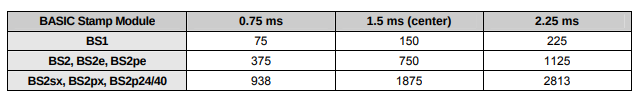
\includegraphics[width=.7\linewidth]{pictures/servo_duty_cycle.png}
    \caption{Valores de \textit{duty cycle} límites según el fabricante \cite{90000005ServomotorParallax}.}
    \label{fig:servo_dtc}
\end{figure}

La conversión en sí consiste en hacer un mapeo del valor de entrada, el cual responde
a la siguiente ecuación (ecuación \ref{eq:map}):

\begin{gather*}
    \left\{\begin{aligned}
        x & \in \left[n, m\right] \\[1ex]
        o & \in \left[k, v\right]    
    \end{aligned}\right. \notag \\[2ex]
    o = \frac{\left(x - n\right) \cdot \left(v - k\right)}{\left(m - n\right) + k} \\ \label{eq:map}
\end{gather*}

Así, el mapeo se haría con una entrada $x \in \left[0, \pi\right]~rad$ y una salida 
$o \in \left[0.75, 2.25\right]~ms$, obteniendo así el \textit{duty cycle} buscado.

Con respecto a trabajar directamente con la posición según el tiempo y el valor del
\textit{duty cycle}, la conversión es algo más compleja y sigue la ecuación \ref{eq:dtc-servo}:

\begin{equation}\label{eq:dtc-servo}
    DTC = \frac{F_{OSC}}{\frac{1000}{ms} \cdot PWM_{Prescaler}}
\end{equation}

De esta manera se pueden generar \textit{duty cycles} que van acorde al tiempo que
ha de durar a nivel alto dicho valor.

Con respecto a la abstracción de \texttt{motor}, se define una estructura que
maneja el \textit{driver} definido anteriormente:

\lstinputlisting[linerange={43-88}, firstnumber=43, caption=, style=C]{pArm-S2/pArm.X/motor/motor.h}

Dicha estructura define:

\begin{itemize}
    \item La dirección de memoria del \textit{driver} del servo.
    \item Un identificador único para el motor.
    \item La duración, si procede, del movimiento que está realizando actualmente el motor.
    \item El ángulo actual, en microsegundos, en el que se encuentra el motor.
    \item \textit{Flag} para indicar si el movimiento actual se ha finalizado.
    \item \textit{Flag} de control indicando si el movimiento es en el sentido de las agujas del reloj o en sentido contrario.
    \item Función que permite iniciar el \textit{timer} dedicado al movimiento del motor.
    \item Función que permite detener el \textit{timer} dedicado al movimiento del motor.
\end{itemize}

El paquete anterior define una interfaz con métodos útiles para permitir el manejo
de los motores:

\lstinputlisting[linerange={90-135}, firstnumber=90, caption=, style=C]{pArm-S2/pArm.X/motor/motor.h}

\LTXtable{\linewidth}{software/s2/motor_table}

Un punto interesante del manejo de la posición de los motores es el método empleado.
Los servomotores que se están empleando no cuentan con ningún tipo de retroalimentación
que indique la posición en la que se encuentra más allá del control que pueda llevar
el desarrollador a nivel de aplicación. Además, el sistema \ac{S2} permite cancelar un
movimiento en ejecución, por lo que es necesario saber en cada instante de tiempo la
posición del motor. Una ventaja que presentan los servomotores es que, si trabajan
dentro de los límites establecidos (no mueven más carga de la especificada, etc.)
presentan una velocidad de giro que puede considerarse constante.

Se plantea entonces el sistema \ac{S2} para manejar de forma precisa el punto
en el que se encuentra el motor. Para ello, se establece una precisión de microsegundo
y se inicializa un contador que es el encargado de llevar el registro del tiempo
que ha pasado desde que un motor ha iniciado su movimiento.

Para ello, se definen tres \textit{timers} que son iniciados independientemente y
cuando un motor comienza a realizar un giro. Todos reciben la dirección de memoria
en la que se encuentra el motor que están manejando y siguen una implementación
similar, la cual se muestra a continuación:

\lstinputlisting[linerange={36-43}, firstnumber=36, caption=, style=C]{pArm-S2/pArm.X/timers/tmr3.c}

El método anterior es simple pero fundamental para llevar el control de la posición:

\begin{enumerate}
    \item Por una parte, se suma cada vez que es invocado el valor $\numprint[\tcmu s]{1.0016}$
    al contador de tiempo propio del \textit{timer}. Esto es debido a que, con la frecuencia
    de oscilación actual no es posible conseguir un valor exacto de $\numprint[\tcmu s]{1}$.
    \item Si la cuenta de tiempo es mayor o igual que la duración del movimiento del
    motor quiere decir que se ha llegado a la posición indicada. Se indica entonces que
    el movimiento ha finalizado, que el servomotor ha llegado a la posición de destino
    y se actualiza la posición actual del motor sumando (o restando) el tiempo que lleva
    activo el \textit{timer} con la posición anterior. Finalmente, detiene el \textit{timer}.
    \item En cualquier caso, desactiva el \textit{flag} de la interrupción para evitar
    entrar múltiples veces en la rutina de tratamiento.
\end{enumerate}

De esta manera, si el usuario decide cancelar el movimiento se tiene de manera
bastante precisa la posición del servomotor en ese instante de tiempo. Tras realizar
un estudio estadístico con 30 muestras\footnote{Se tomaron 30 marcas temporales en las
que el motor se hizo girar una cantidad predefinida de grados (en particular, 90\textdegree),
y se midió el tiempo que se tardaba en realizar dicho movimiento. Se obtuvo una media de
$\overline{x} = \numprint[s]{0.457}$ y una desviación estándar de 
$S(x) \approx \numprint[s]{0.0150748134}$, por lo que se estimó (teniendo en cuenta
el posible fallo humano) que en hacer 
$1\degree \approx \numprint[s]{0.0052452757} \Rightarrow M_{Speed} \approx \numprint[\degree / s]{190.6477479}$.}
(ya que no se encontró ninguna información en la documentación del fabricante)
se estima que la velocidad de giro del motor es:

\begin{equation*}
    M_{Speed} \approx \numprint[\tcmu s / \degree]{5245.27504}
\end{equation*}

Con la relación anterior se pueden establecer \textit{timers} que actúan cada
$\numprint[\mu s]{1.0016}$ para saber con alta precisión el punto aproximado en el
que el motor se encuentra. La precisión se podría mejorar si:

\begin{itemize}
    \item Se cuenta con la velocidad de giro precisa de los motores, dada por el fabricante.
    \item Se incrementa la precisión del \textit{timer} a nivel nanométrico. Esta alternativa
    se planteó pero la interrupción se realizaba con una frecuencia suficientemente elevada
    como para que el sistema se volviera inestable.
\end{itemize}

Finalmente, se encuentra la abstracción de \texttt{planner}. En dicha abstracción se
aúnan todos los motores que componen el brazo en la siguiente estructura:

\lstinputlisting[linerange={39-44}, firstnumber=39, caption=, style=C]{pArm-S2/pArm.X/arm/planner.h}

En dicha estructura se guarda la dirección de memoria de cada uno de los motores
que componen el brazo. La razón de ser de la misma es recoger, de forma ordenada,
la cantidad de motores disponibles y poder utilizarlo a lo largo del \ac{SW}.

La interfaz \texttt{planner} ofrece un nuevo nivel de abstracción sobre los dos
anteriores para poder planificar movimientos completos o bien moviendo los tres
motores del brazo robótico según unos ángulos de entrada 
$\left\{\theta_0, \theta_1, \theta_2\right\}$ o bien mediante la posición en
coordenadas cartesianas del \textit{end--effector}: $P_{ee} = \left\{x, y, z\right\}$.
Además, se ofrecen maneras de conocer la posición exacta tanto en coordenadas angulares
como en coordenadas cartesianas de los tres motores a la vez o del \textit{end--effector},
respectivamente.

Se definen pues los siguientes métodos:

\lstinputlisting[linerange={48-59}, firstnumber=48, caption=, style=C]{pArm-S2/pArm.X/arm/planner.h}

\LTXtable{\linewidth}{software/s2/planner_table}
